% Provenance (never printed): see sources/outline_sources.md (Year 2: mid-latitude cyclones and
% fronts; jets and Rossby waves, descriptive; tropical cyclones; numerical weather prediction,
% principle). Definitions after the NWS glossary and UCAR; cyclogenesis conditions after the NOAA
% AOML FAQ; potential intensity after Gilford (2021, pyPI); conveyor belts after Raveh-Rubin and
% Catto (2019); blocking after Wang and others (2026); predictability after Krishnamurthy (2019),
% Selz and others (2022) and ECMWF. The Lorenz system from figdata/bachelor-2/weather.py; the
% fronts, waves and storms of the examples, exercises and problem are invented, their values
% computed in the Book 4 scratch calculator calc/ch22.py.
\chapter{Weather Systems}\label{ch:b2:weather-systems}

A forecast for four days ahead is now as accurate as a forecast for one day ahead was thirty
years ago, and each decade has added about a day of useful forecast. Yet no forecast of the
weather on a given day, at a given place, is reliable much beyond ten days, and better computers
alone will not push that limit far: the atmosphere amplifies its own small uncertainties. This
chapter describes the weather systems that forecasts follow, the fronts and depressions of the
middle latitudes, the waves of the jet stream and the tropical cyclones, and then the way they
are forecast and why the forecast must stop somewhere.
% ledger: mo:accuracy, bauer:day-per-decade, krish19:predictability

\begin{recall}
\textbf{From the school volumes}: air masses, fronts, cold and warm fronts, depressions and
anticyclones, isobars and weather forecasts; the tropical cyclone, its eye and eyewall, the
Saffir--Simpson scale. \textbf{From the Year 1 volume}: the pressure-gradient force, the
Coriolis parameter $f = 2\Omega\sin\varphi$, geostrophic balance, cyclones and anticyclones, the
three cells, the westerlies and the jet streams. \textbf{From the physics books}: heat engines
and the efficiency of a Carnot cycle. \textbf{From \cref{ch:b2:atmospheric-thermodynamics}}:
saturation, the \omterm{def:b2:atmospheric-thermodynamics:moist-adiabat}{moist adiabat}, $\theta_e$, \omterm{def:b2:atmospheric-thermodynamics:instability}{conditional instability} and CAPE.
\end{recall}

\section{Fronts}\label{sec:b2:weather-systems:fronts}

The school volumes drew fronts as lines on a map. A front is the line where a sloping boundary
between two air masses meets the ground, and its weather comes from that slope.

\begin{definition}[Frontal surface; stationary front; occluded front]\label{def:b2:weather-systems:fronts}
The \emph{frontal surface}\index{frontal surface} of a front is the sloping boundary between
the two air masses, the denser, colder one lying beneath as a wedge; the front on the map is its
intersection with the ground. A \emph{stationary front}\index{stationary front} is a front
that moves very slowly or not at all. An \emph{occluded front}\index{occluded front} is a
composite of two fronts, formed when a cold front overtakes a warm or stationary front.
\end{definition}
% ledger: nws4:front, nws4:stationary, nws4:occluded

A \omterm{def:b2:weather-systems:fronts}{stationary front} forms when neither air mass can push the other, the winds blowing along the
front rather than across it; it can stay for days, cloudy and wet, before moving again as a cold
or a warm front. On a map it alternates the blue triangles of a cold front, pointing towards the
warm air, with the red semicircles of a warm front, pointing towards the cold air. An \omterm{def:b2:weather-systems:fronts}{occluded
front} is drawn in purple with both symbols on the same side. When the air behind the cold front
is the colder, it slides under the warm front and lifts it aloft, a cold occlusion; when the air
ahead of the warm front is the colder, the cold front rides up over it, a warm occlusion.
% ledger: ucar4:stationary-occluded, nws4:occluded

How steep is a \omterm{def:b2:weather-systems:fronts}{frontal surface}? The answer joins the hydrostatic balance to the geostrophic
balance of the Year 1 volume.

\begin{proposition}[Slope of a frontal surface]\label{prop:b2:weather-systems:slope}
Let a \omterm{def:b2:weather-systems:fronts}{frontal surface} separate cold air at the temperature $T_c$ from warm air at $T_w$, with
geostrophic winds $v_c$ and $v_w$ along the front. Take the axis $x$ across the front towards the
cold air and the axis $y$ along it, so that $(x, y, z)$ is right-handed. Then the \omterm{def:b2:weather-systems:fronts}{frontal
surface} rises towards the cold air with the slope
\[
  \tan\alpha \approx \frac{f\,\bar T\,(v_c - v_w)}{g\,(T_w - T_c)},
\]
where $\bar T$ is the mean temperature. A \omterm{def:b2:weather-systems:fronts}{frontal surface} in balance needs a jump of the wind
along it, $v_c > v_w$: the wind turns cyclonically across the front.
\end{proposition}

\begin{proof}
The pressure is continuous across the \omterm{def:b2:weather-systems:fronts}{frontal surface}, so its change along the surface is the
same computed on either side: $\partial_x p_c\,\mathrm{d}x + \partial_z p_c\,\mathrm{d}z =
\partial_x p_w\,\mathrm{d}x + \partial_z p_w\,\mathrm{d}z$. On each side $\partial_z p = -\rho g$
(hydrostatic balance) and $\partial_x p = \rho f v$ (geostrophic balance). Hence
$\rho_c f v_c\,\mathrm{d}x - \rho_c g\,\mathrm{d}z = \rho_w f v_w\,\mathrm{d}x - \rho_w
g\,\mathrm{d}z$, and
\[
  \frac{\mathrm{d}z}{\mathrm{d}x} = \frac{f(\rho_c v_c - \rho_w v_w)}{g(\rho_c - \rho_w)} .
\]
At the same pressure, $\rho \propto 1/T$, so $\rho_c - \rho_w \approx \bar\rho\,(T_w -
T_c)/\bar T$; in the numerator the small difference of the densities can be neglected, which
gives the formula. The cold air lies beneath, so the surface rises towards it, $\mathrm{d}z/
\mathrm{d}x > 0$, and $v_c > v_w$. With $x$ towards the cold air, the relative vorticity
$\partial v/\partial x$ across the front is then positive: cyclonic.
\end{proof}

\begin{example}[A typical slope]\label{ex:b2:weather-systems:slope}
At \ang{45} N, $f = \qty{1.03e-4}{s^{-1}}$. Across a front with $\bar T = \qty{280}{K}$, a
temperature contrast of \qty{5}{K} and a wind that changes by \qty{10}{m/s} along it, $\tan\alpha
= 1.03 \times 10^{-4} \times 280 \times 10/(9.81 \times 5) = 0.0059$, about 1 in 170: the
\omterm{def:b2:weather-systems:fronts}{frontal surface} reaches a height of \qty{1}{km} some \qty{170}{km} from the front on the ground.
A sharper wind shift gives a steeper surface; a stronger temperature contrast, a gentler one.
\end{example}

Real fronts have slopes of this order, and the shallow wedge explains their weather. Ahead of a
warm front, the warm air glides up a gentle slope for hundreds of kilometres: high clouds,
cirrus and cirrostratus, arrive first, then altostratus, and the clouds thicken and lower until
rain sets in near the front. A cold front, steeper and faster, up to twice as fast as a warm
front, lifts the warm air abruptly: cumulus and cumulonimbus, showers, gusts and a sudden fall
of temperature, with pressure that stops falling and starts rising as the front passes. A front
where the warm air descends the \omterm{def:b2:weather-systems:fronts}{frontal surface} instead of rising up it is called a katafront.
% ledger: ucar:warm-front, ucar:cold-front, nws4:front

\begin{omfigure}
\centering
\begin{tikzpicture}[font=\scriptsize, >=Stealth, x=1cm, y=1cm]
% air masses
\fill[omCold!12] (0,0) -- (0,3.4) .. controls (1.6,2.2) and (3.2,0.8) .. (4,0) -- cycle;
\fill[omCold!12] (9.6,0) .. controls (11,0.6) and (12.6,1.5) .. (14,2.4) -- (14,0) -- cycle;
\fill[omWarm!8] (4,0) .. controls (3.2,0.8) and (1.6,2.2) .. (0,3.4) -- (0,4.8) -- (14,4.8)
  -- (14,2.4) .. controls (12.6,1.5) and (11,0.6) .. (9.6,0) -- cycle;
% frontal surfaces
\draw[omCold, thick] (4,0) .. controls (3.2,0.8) and (1.6,2.2) .. (0,3.4);
\draw[omWarm, thick] (9.6,0) .. controls (11,0.6) and (12.6,1.5) .. (14,2.4);
% clouds
\fill[black!18, draw=black!45] (3.75,0.5) .. controls (3.5,1.8) and (3.7,3.2) .. (3.9,3.9)
  .. controls (3.2,4.15) and (3.0,4.5) .. (3.4,4.6) -- (5.8,4.6) .. controls (6.1,4.45) and
  (5.7,4.15) .. (5.1,3.9) .. controls (5.3,3.0) and (5.4,1.6) .. (5.05,0.5) -- cycle;
\node[align=center] at (4.45,2.6) {cumulo-\\nimbus};
\fill[black!15, draw=black!40] (9.6,0.35) .. controls (10.4,0.75) and (11.2,1.05) .. (11.9,1.25)
  -- (11.9,1.75) .. controls (11,1.6) and (10.2,1.35) .. (9.4,0.95) -- cycle;
\node at (10.75,1.25) [rotate=21] {nimbostratus};
\fill[black!10, draw=black!35] (11.9,1.35) .. controls (12.3,1.55) and (12.7,1.75) .. (13.0,1.9)
  -- (13.0,2.25) .. controls (12.6,2.1) and (12.2,1.95) .. (11.9,1.85) -- cycle;
\node[anchor=south] at (12.45,2.15) {altostratus};
\draw[black!40, line width=1.6pt] (12.9,2.75) -- (13.9,3.05);
\node[anchor=south] at (13.35,3.05) {cirrostratus};
\foreach \x in {12.2,12.7,13.2,13.7} {\draw[black!40, thick] (\x,3.95) .. controls (\x+0.15,4.05) .. (\x+0.35,3.9);}
\node[anchor=south] at (13.0,4.05) {cirrus};
% rain
\foreach \x in {3.95,4.25,4.55,4.85} {\draw[omCold!70, dashed] (\x,0.45) -- (\x-0.12,0.02);}
\foreach \x in {9.8,10.2,10.6,11.0,11.4} {\draw[omCold!70, dashed] (\x,0.55) -- (\x-0.12,0.02);}
% ground and labels
\draw[thick] (0,0) -- (14,0);
\node at (1.2,0.8) {cold air};
\node at (7.0,2.4) {warm sector};
\node at (12.8,0.55) {cold air};
\node[anchor=north, omCold] at (4,-0.05) {cold front};
\node[anchor=north, omWarm] at (9.6,-0.05) {warm front};
\draw[->, thick] (6.0,0.55) -- (7.2,0.55) node[right] {fronts move east};
\draw[->, black!60] (5.8,1.1) .. controls (7.0,1.4) and (9.5,2.0) .. (12.2,3.3);
\node[black!60, rotate=13] at (8.4,2.0) {warm air glides up};
\end{tikzpicture}
\par\smallskip{\small A cross-section through a cold front and a warm front, west on the left
(schematic: the vertical scale is exaggerated about a hundred times, and the cold front is drawn
steeper than the warm front). Cloud names and sequences as in the text.}
\end{omfigure}
% ledger: ucar:warm-front, ucar:cold-front

\section{Extratropical cyclones}\label{sec:b2:weather-systems:cyclones}

\begin{definition}[Extratropical cyclone; polar-front model; cyclogenesis]\label{def:b2:weather-systems:cyclones}
An \emph{extratropical cyclone}\index{extratropical cyclone} is a cyclone of the middle and high
latitudes, often some \qty{2000}{km} across, which usually contains fronts, a cold front trailing
for hundreds of kilometres towards the equator. The \emph{polar-front model}\index{polar-front model}
describes its life as a wave that grows on the polar front, the long front between polar
and tropical air. \emph{Cyclogenesis}\index{cyclogenesis} is the formation or the intensification
of a cyclone.
\end{definition}
% ledger: nws4:extratropical, nws4:polar-front

The model follows a cyclone through four stages, as the figure below draws them. A \omterm{def:b2:weather-systems:fronts}{stationary
front} separates cold air moving west on its polar side from warm air moving east on its
equatorial side. A disturbance bends the front into a wave; the pressure falls at its crest, a
low forms, and the front east of the low advances poleward as a warm front while the front west
of it advances equatorward as a cold front. Between them lies the warm sector. The cold front
moves faster than the warm front, the warm sector narrows, and the cold front overtakes the warm
front near the low: the occlusion spreads outward from the centre, lifting the warm air off the
ground, and the cyclone, cut off from its supply of warm air, fills and dies. The point where the
three fronts meet is called the triple point. On satellite images a mature cyclone shows a
comma-shaped cloud, and a dry slot of clear air wrapping into its southern and eastern side.
% ledger: nws4:extratropical, nws4:occluded, ucar:cold-front

\begin{omfigure}
\centering
\begin{tikzpicture}[font=\scriptsize, >=Stealth]
% (a) stationary front
\begin{scope}[shift={(0,4.1)}]
\draw[black!30] (0,0) rectangle (6.4,3.4);
\node[anchor=north west] at (0,3.4) {\textbf{a}\enspace stationary front};
\draw[stationary front] (6.1,1.6) -- (0.3,1.6);
\draw[->, black!60] (4.2,2.5) -- (2.2,2.5); \node[black!60] at (3.2,2.8) {cold air};
\draw[->, black!60] (2.2,0.7) -- (4.2,0.7); \node[black!60] at (3.2,0.4) {warm air};
\end{scope}
% (b) open wave
\begin{scope}[shift={(6.9,4.1)}]
\draw[black!30] (0,0) rectangle (6.4,3.4);
\node[anchor=north west] at (0,3.4) {\textbf{b}\enspace a wave and a low};
\fill[omWarm!10] (3.0,1.9) .. controls (3.9,1.75) and (4.8,1.55) .. (6.0,1.4) -- (6.0,0.2)
  -- (1.3,0.2) .. controls (2.0,0.9) and (2.6,1.4) .. (3.0,1.9) -- cycle;
\draw[black!45] (3.0,1.9) ellipse (0.55 and 0.4);
\draw[black!45] (3.0,1.9) ellipse (1.05 and 0.75);
\draw[warm front] (3.0,1.9) .. controls (3.9,1.75) and (4.8,1.55) .. (6.0,1.4);
\draw[cold front] (3.0,1.9) .. controls (2.6,1.4) and (2.0,0.9) .. (1.3,0.2);
\node[font=\small\bfseries, omWarm!70!black] at (2.7,2.15) {L};
\node at (4.5,0.75) {warm sector};
\end{scope}
% (c) mature
\begin{scope}[shift={(0,0)}]
\draw[black!30] (0,0) rectangle (6.4,3.4);
\node[anchor=north west] at (0,3.4) {\textbf{c}\enspace mature cyclone};
\fill[omWarm!10] (3.0,1.9) .. controls (3.9,1.7) and (4.8,1.5) .. (6.0,1.25) -- (6.0,0.2)
  -- (3.3,0.2) .. controls (3.3,0.8) and (3.2,1.45) .. (3.0,1.9) -- cycle;
\draw[black!45] (3.0,1.9) ellipse (0.5 and 0.36);
\draw[black!45] (3.0,1.9) ellipse (0.95 and 0.66);
\draw[black!45] (3.0,1.9) ellipse (1.4 and 0.95);
\draw[warm front] (3.0,1.9) .. controls (3.9,1.7) and (4.8,1.5) .. (6.0,1.25);
\draw[cold front] (3.0,1.9) .. controls (3.2,1.45) and (3.3,0.8) .. (3.3,0.2);
\node[font=\small\bfseries, omWarm!70!black] at (2.7,2.15) {L};
\node at (4.9,0.65) {warm sector};
\end{scope}
% (d) occluded
\begin{scope}[shift={(6.9,0)}]
\draw[black!30] (0,0) rectangle (6.4,3.4);
\node[anchor=north west] at (0,3.4) {\textbf{d}\enspace occlusion};
\fill[omWarm!10] (4.0,1.55) .. controls (4.6,1.45) and (5.3,1.3) .. (6.1,1.1) -- (6.1,0.2)
  -- (4.6,0.2) .. controls (4.5,0.7) and (4.3,1.2) .. (4.0,1.55) -- cycle;
\draw[black!45] (2.5,1.95) ellipse (0.5 and 0.36);
\draw[black!45] (2.5,1.95) ellipse (0.95 and 0.66);
\draw[black!45] (2.5,1.95) ellipse (1.45 and 0.95);
\draw[occluded front] (2.5,1.95) .. controls (3.0,1.9) and (3.6,1.75) .. (4.0,1.55);
\draw[warm front] (4.0,1.55) .. controls (4.6,1.45) and (5.3,1.3) .. (6.1,1.1);
\draw[cold front] (4.0,1.55) .. controls (4.3,1.2) and (4.5,0.7) .. (4.6,0.2);
\node[font=\small\bfseries, omWarm!70!black] at (2.2,2.2) {L};
\node[anchor=north east, align=right, fill=white, inner sep=1pt] at (3.9,1.3) {triple\\point};
\fill (4.0,1.55) circle (0.6mm);
\end{scope}
\end{tikzpicture}
\par\smallskip{\small The life of an \omterm{def:b2:weather-systems:cyclones}{extratropical cyclone} in the \omterm{def:b2:weather-systems:cyclones}{polar-front model}, Northern
Hemisphere, north at the top (schematic): a \omterm{def:b2:weather-systems:fronts}{stationary front} (a); a wave with a low at its crest,
a warm front and a cold front and the warm sector between them (b); the cold front catches up
(c); the \omterm{def:b2:weather-systems:fronts}{occluded front} grows from the centre (d). Black ellipses: isobars.}
\end{omfigure}
% ledger: nws4:occluded, nws4:extratropical, ucar4:stationary-occluded

The fronts of the model are only the surface trace of the airflows of the cyclone, which
meteorologists describe as three streams: a warm conveyor belt, the moist air that rises from the
warm sector ahead of the cold front; a cold conveyor belt on the cold side of the fronts; and a
dry intrusion, a stream of air from the upper troposphere, sometimes from the lowest
stratosphere, that descends towards the surface behind the cold front and fans out near the
ground.
% ledger: rr19:conveyor

Where does the energy of a cyclone come from? Not from latent heat alone, as in a thunderstorm,
but from the contrast of temperature between polar and tropical air. Mid-latitude cyclones
strengthen in baroclinic zones, where the temperature changes horizontally on a surface of
constant pressure and the wind changes with height. A growing cyclone carries warm air poleward
and upward and cold air equatorward and downward: it lowers the centre of mass of the
atmosphere and converts potential energy into the kinetic energy of its winds. The Year~3
volume studies that conversion.
% ledger: nws4:extratropical

\begin{omfigure}
\centering
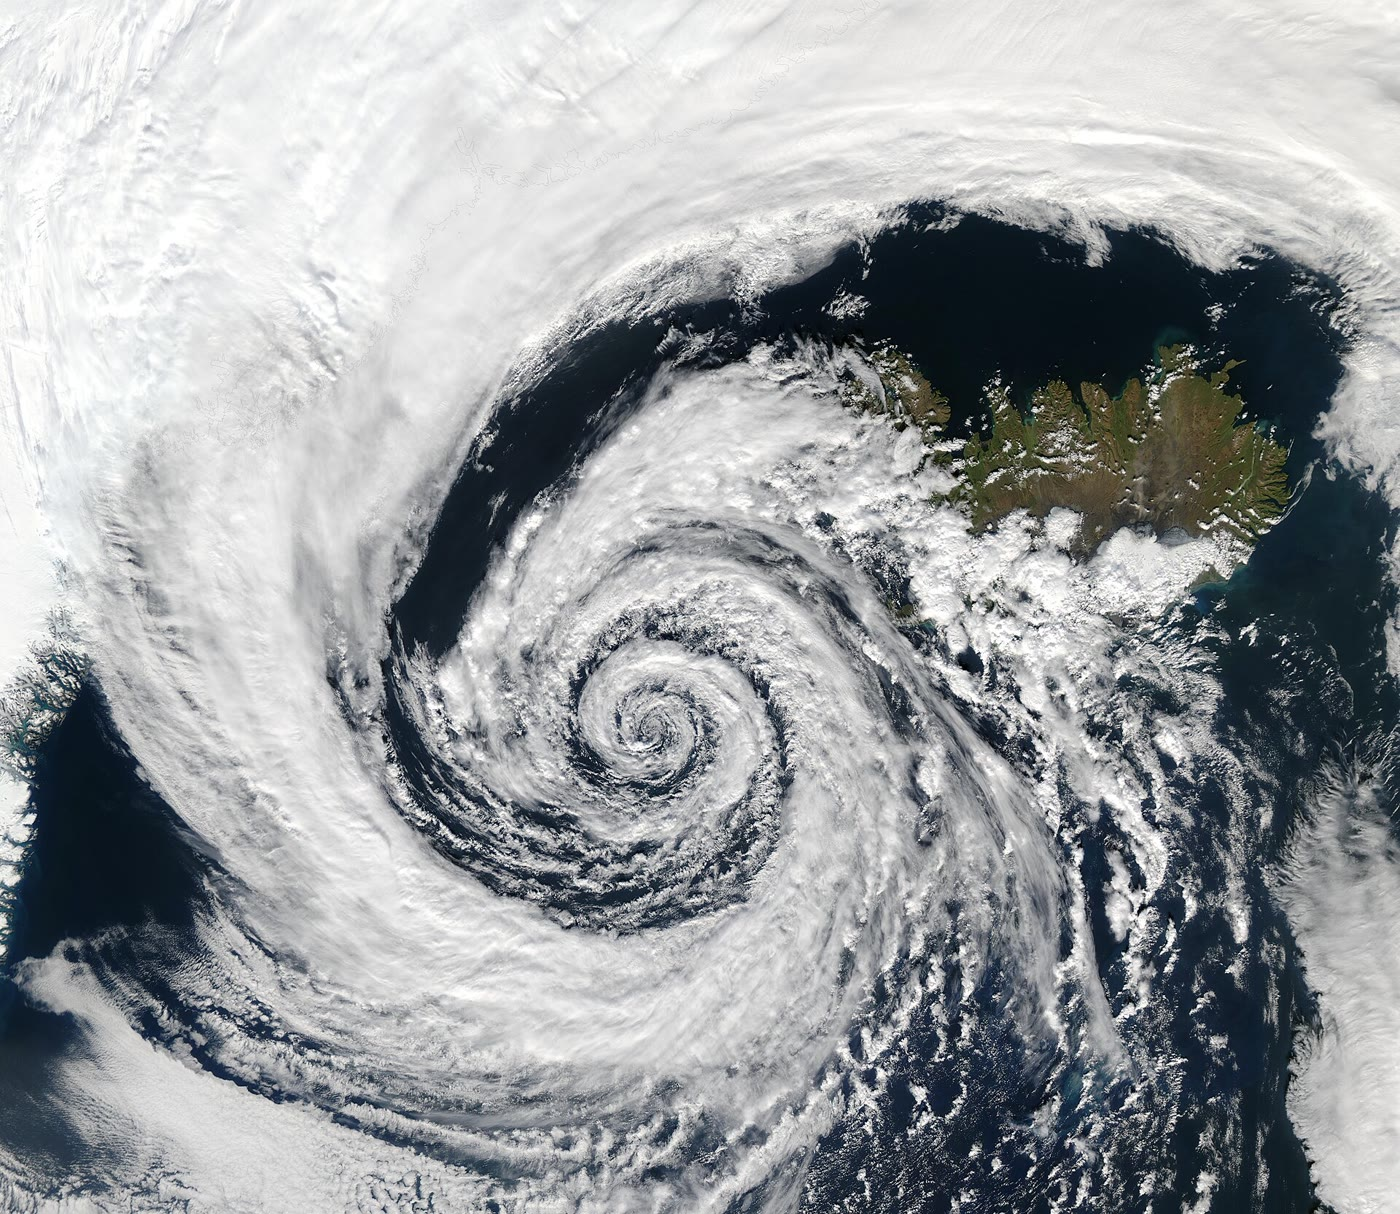
\includegraphics[width=0.58\linewidth]{images/book4/b2-22-iceland-low.jpg}
\par\smallskip{\small A deep low off the south-west coast of Iceland, 4 September 2003, seen by
the MODIS instrument of NASA's Aqua satellite: the cloud bands spiral into the centre. (NASA
Goddard Space Flight Center, MODIS Rapid Response Team, Jacques Descloitres, public domain, via
Wikimedia Commons.)}
\end{omfigure}

\section{Jet streams and Rossby waves}\label{sec:b2:weather-systems:rossby}

Cyclones are not scattered at random. The polar jet, the fast core of the westerlies above the
polar front, goes with the position and the motion of the highs and lows of the middle
latitudes; it is fastest along its jet streaks, the stretches where its wind speed peaks, and it
does not circle the pole as a ring: it meanders.
% ledger: nws4:polar-front, nws4:jet-streak

\begin{definition}[Rossby wave; upper-level trough and ridge]\label{def:b2:weather-systems:rossby}
A \emph{Rossby wave}\index{Rossby wave} is a wave of the westerly flow of the upper troposphere,
a series of troughs and ridges thousands of kilometres long with a large north--south amplitude.
An \emph{upper-level trough}\index{upper-level trough} is an elongated region of relatively low
pressure in such a wave, where the flow bends towards the equator; an \emph{upper-level
ridge}\index{upper-level ridge} is an elongated region of relatively high pressure, where it
bends towards the pole.
\end{definition}
% ledger: nws4:rossby

\omterm{def:b2:weather-systems:rossby}{Rossby waves} exist because the Coriolis parameter grows towards the pole. Air pushed poleward
finds a larger $f$ and, conserving its absolute vorticity, turns back towards the equator; air
pushed equatorward turns back towards the pole. The rate at which $f$ grows northward,
$\beta = \mathrm{d}f/\mathrm{d}y = 2\Omega\cos\varphi/a$ with $a$ the radius of the Earth, sets
their speed. The Year~3 volume derives, from the conservation of vorticity, the phase speed of a
wave of wavelength $\lambda$ in a uniform westerly wind $U$:
\[
  c = U - \frac{\beta}{k^2}, \qquad k = \frac{2\pi}{\lambda} .
\]
Admit it here. Relative to the air, every \omterm{def:b2:weather-systems:rossby}{Rossby wave} moves west, and the longer the wave, the
faster; the wind carries it east. Short waves are carried east almost at the speed of the wind,
long ones drift slowly, stand still, or even move west.
% ledger: earth:Trot, earth:Rmean

\begin{example}[Three waves at 45° N]\label{ex:b2:weather-systems:rossby}
With $\Omega = \qty{7.292e-5}{s^{-1}}$ (a sidereal day of \qty{23.9345}{h}) and $a =
\qty{6371}{km}$, $\beta = \qty{1.62e-11}{m^{-1}.s^{-1}}$ at \ang{45} N. In a westerly of
\qty{15}{m/s}, a wave of \qty{4000}{km} has $\beta/k^2 = \qty{6.6}{m/s}$ and moves east at
\qty{8.4}{m/s}; one of \qty{6000}{km} has $\beta/k^2 = \qty{14.8}{m/s}$ and barely moves, at
\qty{0.2}{m/s}; one of \qty{8000}{km} moves west at \qty{11.2}{m/s}.
\end{example}
% ledger: earth:Trot, earth:Rmean

The troughs of the long waves move slowly and last long; the short waves that travel through
them, shortwave troughs, induce rising air ahead of them, on their eastern side, where the
surface pressure falls and lows develop. A trough whose axis tilts from south-east to north-west
is often a sign of a developing or intensifying system.
% ledger: nws4:rossby

\begin{omfigure}
\centering
\begin{tikzpicture}[font=\scriptsize, >=Stealth]
\foreach \lat/\pa in {30/-72, 45/-72, 60/-108} {
  \pgfmathsetmacro{\r}{6.0*tan((90-\lat)/2)}
  \draw[black!25] (0,0) circle (\r);
  \node[black!50, fill=white, inner sep=1pt] at (\pa:\r) {\ang{\lat} N};
}
\fill (0,0) circle (0.6mm);
\node[anchor=north, black!60] at (0,-0.08) {North Pole};
\draw[ocBlue, very thick, smooth, samples=241, domain=0:360]
  plot ({6.0*tan((90-(47+11*cos(5*\x)))/2)*cos(\x)}, {6.0*tan((90-(47+11*cos(5*\x)))/2)*sin(\x)});
\foreach \a in {18, 90, 162, 234, 306} {
  \pgfmathsetmacro{\ra}{6.0*tan((90-(47+11*cos(5*\a)))/2)}
  \pgfmathsetmacro{\rb}{6.0*tan((90-(47+11*cos(5*(\a+2))))/2)}
  \draw[ocBlue, very thick, -{Stealth[length=2.6mm]}] (\a:\ra) -- (\a+2:\rb);
}
\pgfmathsetmacro{\rt}{6.0*tan((90-36)/2)}
\node[anchor=216, ocRed!80!black, inner sep=2pt] at (36:\rt) {trough};
\node[anchor=0, ocRed!80!black, inner sep=2pt] at (180:\rt) {trough};
\pgfmathsetmacro{\rr}{6.0*tan((90-58)/2)}
\node[anchor=72, ocRed!80!black, inner sep=3pt] at (72:\rr) {ridge};
\end{tikzpicture}
\par\smallskip{\small \omterm{def:b2:weather-systems:rossby}{Rossby waves} in the jet stream seen from above the North Pole (schematic):
five waves round the hemisphere, troughs reaching towards the equator and ridges towards the
pole. The jet flows eastward, anticlockwise seen from above the pole (arrows). Latitude circles
drawn as on a polar stereographic map.}
\end{omfigure}
% ledger: nws4:rossby

Sometimes the pattern stops moving altogether.

\begin{definition}[Atmospheric blocking]\label{def:b2:weather-systems:blocking}
\emph{Atmospheric blocking}\index{atmospheric blocking} is a large, persistent and nearly
stationary high-pressure system, sometimes paired with a low, that interrupts the normal eastward
flow of the jet stream. Methods of detecting blocks almost all require it to last at least five
days.
\end{definition}
% ledger: wang26:blocking

A block diverts the jet and the cyclones around it and holds the same weather over the same
region for days: blocks bring heat waves, droughts, wildfires, cold spells and floods to the
middle latitudes. In late June and early July 2021 a strong block led to the heat wave of the
Pacific Northwest of North America, which caused more than a thousand deaths. The physical
processes behind blocking are still not well understood, and numerical models struggle to
reproduce how often blocks occur and how long they last.
% ledger: wang26:blocking, wang26:gaps

\section{Tropical cyclones}\label{sec:b2:weather-systems:tropical}

Tropical cyclones have no fronts and no temperature contrast to feed on. They draw their energy
from the warm ocean, through the latent heat of the water they evaporate, as \cref{ch:b2:atmospheric-thermodynamics}
measured it. Six conditions favour their formation: ocean water of at least \qty{26.5}{\celsius}
through a depth of the order of \qty{50}{m}; an atmosphere that cools fast enough with height to
be unstable for moist convection; a moist middle troposphere, around \qty{5}{km}; a distance of
at least about \qty{500}{km} from the equator, so that the Coriolis force can hold the low in
balance; a pre-existing disturbance near the surface; and weak vertical wind shear, below about
\qty{10}{m/s} between the surface and the upper troposphere. They are necessary but not
sufficient: many disturbances that meet them never develop.
% ledger: aoml:tc-genesis

Once formed, a tropical cyclone is a heat engine. Air spirals inward over the sea at almost
constant temperature, gaining heat and moisture from the ocean; in the eyewall it rises
adiabatically; in the outflow near the tropopause it loses heat by radiation at a low,
almost constant temperature; and it sinks again far from the centre, completing a cycle that
resembles that of Carnot. The work of the cycle drives the winds against the friction of the sea
surface.
% ledger: gilford21:pi

\begin{omfigure}
\centering
\begin{tikzpicture}[font=\scriptsize, >=Stealth, x=1cm, y=1cm]
% sea and axis
\fill[ocBlue!12] (0,-0.35) rectangle (12.5,0);
\draw[thick, ocBlue!70!black] (0,0) -- (12.5,0);
\node[anchor=north west, ocBlue!70!black] at (8.6,-0.02) {warm sea, $T_s$};
\draw[dashed, black!50] (0,-0.35) -- (0,4.9);
\node[anchor=south, black!60] at (0,4.9) {centre};
% eyewall cloud and outflow cloud
\fill[black!14, draw=black!40] (0.9,0.25) .. controls (0.7,1.8) and (0.75,3.3) .. (0.95,4.2)
  .. controls (3.5,4.55) and (7.0,4.45) .. (9.5,4.2) .. controls (7.0,3.9) and (3.6,3.85)
  .. (2.1,3.7) .. controls (1.95,2.6) and (1.9,1.4) .. (2.0,0.25) -- cycle;
\node[black!60] at (0.45,2.0) [rotate=90] {eye};
\draw[black!50] (1.9,1.1) -- (2.45,1.1) node[anchor=west, black!70] {eyewall cloud};
% the cycle
\draw[->, very thick, ocRed] (11.4,0.3) -- (2.3,0.3);
\draw[->, very thick, ocRed] (1.45,0.45) .. controls (1.4,1.6) and (1.45,3.0) .. (1.75,4.0);
\draw[->, very thick, ocBlue] (2.2,4.25) -- (11.2,4.25);
\draw[->, very thick, ocBlue] (11.6,4.05) .. controls (11.75,2.8) and (11.75,1.5) .. (11.6,0.45);
\fill (11.6,0.3) circle (0.7mm) node[right=2pt] {A};
\fill (1.45,0.3) circle (0.7mm) node[left=2pt] {B};
\fill (1.8,4.25) circle (0.7mm) node[above left=1pt] {C};
\fill (11.6,4.25) circle (0.7mm) node[above right=1pt] {D};
\node[anchor=south, align=center] at (6.5,0.35) {A$\to$B: inflow over the sea at about $T_s$,
  taking up heat and moisture};
\node[anchor=west, align=left] at (2.25,2.3) {B$\to$C: rises in the eyewall,\\without
  exchanging heat (moist adiabat)};
\node[anchor=south, align=center] at (6.5,4.62) {C$\to$D: outflow near the tropopause at about
  $T_o$, losing heat by radiation};
\node[anchor=east, align=right] at (11.45,2.3) {D$\to$A: sinks far\\from the centre};
\end{tikzpicture}
\par\smallskip{\small The heat engine of a tropical cyclone, a vertical section from the centre
outwards (schematic, not to scale): heat is taken up at the temperature of the sea surface
(A$\to$B) and given off at the much lower temperature of the outflow (C$\to$D), as in a Carnot
cycle.}
\end{omfigure}
% ledger: gilford21:pi

\begin{proposition}[Potential intensity]\label{prop:b2:weather-systems:pi}
\index{potential intensity}
The \emph{\omterm{prop:b2:weather-systems:pi}{potential intensity}} of a tropical cyclone, the maximum wind speed near the surface that
the ocean and atmosphere around it can sustain, is approximately given by
\[
  V_{\max}^2 = \frac{C_k}{C_D}\,\frac{T_s - T_o}{T_o}\,\bigl(h_o^* - h^*\bigr),
\]
where $T_s$ is the temperature of the sea surface, $T_o$ the temperature of the outflow, $C_k/C_D$
the ratio of the exchange coefficients of enthalpy and momentum between the sea and the air,
usually taken as 0.9, and $h_o^* - h^*$ the excess of $c_pT + gz + Lq$ at saturation at the sea
surface over its saturation value in the air above the boundary layer (admitted).
\end{proposition}
% ledger: gilford21:pi

The fraction $(T_s - T_o)/T_o$ is not the Carnot efficiency $(T_s - T_o)/T_s$ of the physics
books: it is larger by the factor $T_s/T_o$, because the friction that dissipates the work heats
the inflowing air near the sea surface, and that heat is used again by the engine. The last
factor is the fuel. In a tropical atmosphere whose temperature follows the \omterm{def:b2:atmospheric-thermodynamics:moist-adiabat}{moist adiabat} of its
boundary-layer air, $h^*$ is the value of $c_pT + gz + Lq$ in that air, and $h_o^* - h^*$
measures how far the air over the sea is from saturation at the temperature of the sea:
\[
  h_o^* - h^* \approx c_p\,(T_s - T_a) + L\,(q_s^* - q_a),
\]
with $T_a$ and $q_a$ the temperature and \omterm{def:b2:atmospheric-thermodynamics:moist-air}{specific humidity} of the air near the surface and
$q_s^*$ the saturation \omterm{def:b2:atmospheric-thermodynamics:moist-air}{specific humidity} at the sea-surface temperature.
% ledger: gilford21:pi

\begin{example}[A potential intensity]\label{ex:b2:weather-systems:pi}
Over a sea at \qty{29}{\celsius} the air at \qty{1015}{hPa} is at \qty{28}{\celsius} with a
relative humidity of \qty{80}{\percent}, and the outflow is at \qty{200}{K}, a typical annual
mean over the warm tropical oceans. By \cref{prop:b2:atmospheric-thermodynamics:es,prop:b2:atmospheric-thermodynamics:humidity},
$e_s(\qty{29}{\celsius}) = \qty{41.0}{hPa}$, so $q_s^* = \qty{25.5}{g/kg}$, and the air, with
$e = 0.8 \times \qty{38.7}{hPa}$, has $q_a = \qty{19.2}{g/kg}$. Then $h_o^* - h^* = 1004.5 \times
1 + 2.501 \times 10^6 \times 0.0063 = \qty{16.8}{kJ/kg}$, the factor $(T_s - T_o)/T_o$ is
$(302.15 - 200)/200 = 0.511$, and $V_{\max} = \sqrt{0.9 \times 0.511 \times 16\,800} =
\qty{88}{m/s}$.
\end{example}
% ledger: gilford21:pi

The strongest storms come close to such values: the top of the Saffir--Simpson scale, category
5, starts at \qty{70}{m/s}, and five recent storms have exceeded \qty{86}{m/s}. Most storms
rarely reach their \omterm{prop:b2:weather-systems:pi}{potential intensity}: real storms are seldom in the steady state the theory
assumes, and the theory leaves out vertical wind shear, dry air drawn into the storm and the
sinking of the air around it, which weaken a storm.
% ledger: wk24:scale, gilford21:limits, aoml:tc-weaken

\begin{omfigure}
\centering
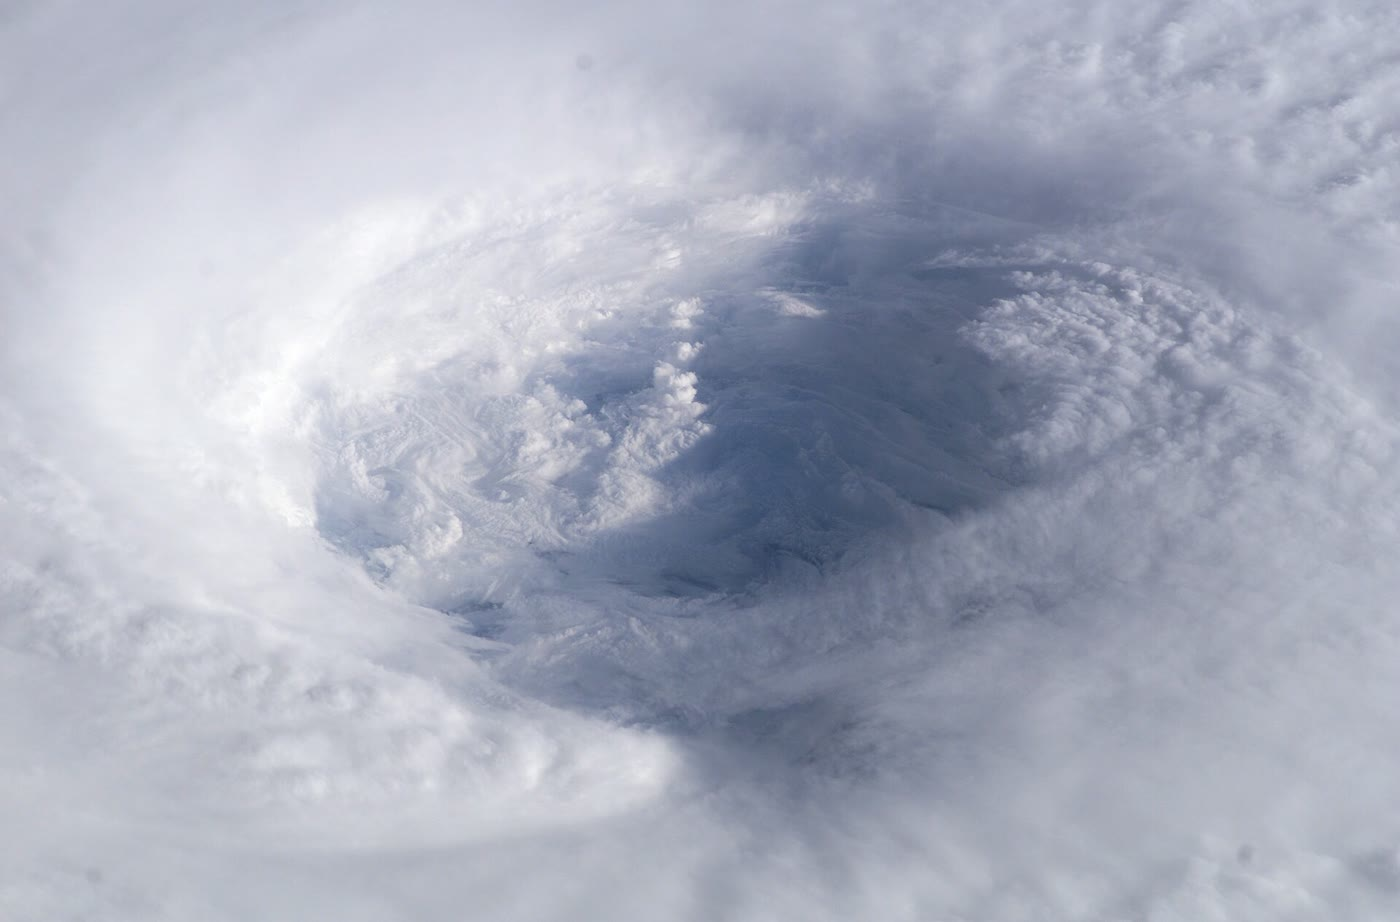
\includegraphics[width=0.62\linewidth]{images/book4/b2-22-isabel-eye.jpg}
\par\smallskip{\small The eye of Hurricane Isabel, 13 September 2003, photographed from the
International Space Station: the eyewall falls like a stadium to the low clouds in the eye.
(NASA astronaut Ed Lu, public domain, via Wikimedia Commons.)}
\end{omfigure}

\section{Numerical weather prediction}\label{sec:b2:weather-systems:nwp}

\begin{definition}[Numerical weather prediction; data assimilation; ensemble forecast; predictability limit]\label{def:b2:weather-systems:nwp}
\emph{Numerical weather prediction}\index{numerical weather prediction} is forecasting by
computer: the equations that govern the motion, the energy and the water of the atmosphere are
integrated forward in time from its observed state. \emph{Data assimilation}\index{data assimilation}
combines the latest observations with a short-range forecast from earlier
observations to obtain the best estimate of the present state, the analysis, from which the
forecast starts. An \emph{ensemble forecast}\index{ensemble forecast} is a set of forecasts run
from slightly different initial states, and with slightly different versions of the model, to
show the range of possible weather and its likelihood. The \emph{predictability
limit}\index{predictability limit} is the time beyond which a forecast of the state of the
weather is no better than a guess from climate, because the errors of the initial state have
grown as large as the differences between any two states of the atmosphere.
\end{definition}
% ledger: nws4:nwp, ecmwf4:da, ecmwf4:ens-fs, krish19:predictability

The first numerical forecast was computed in 1950 on ENIAC, one of the first electronic
computers. A global model today divides the atmosphere into a grid of cells some kilometres
across and starts from an analysis that blends observations from weather stations, aircraft,
radiosondes, ships, buoys and, above all, satellites, which bring the largest contribution to the
skill of global forecasts. At one large forecast centre the ensemble
has 51 members, a control run and 50 perturbed ones, at a resolution of about \qty{9}{km}, run
twice a day to 15 days ahead.
% ledger: krish19:predictability, ecmwf4:da, ecmwf4:ens

Why perturb a forecast that could start from the best analysis? Because the atmosphere is
chaotic, sensitive to its initial state. A system of three variables, published in 1963, shows it
at the smallest scale.

\begin{proposition}[The Lorenz system]\label{prop:b2:weather-systems:lorenz}
The system
\[
  \dot x = \sigma(y - x), \qquad \dot y = x(r - z) - y, \qquad \dot z = xy - bz,
\]
with $\sigma = 10$, $r = 28$ and $b = 8/3$, has the following properties.
\begin{enumerate}
  \item Its fixed points are the origin and $C_\pm = \bigl(\pm\sqrt{b(r - 1)}, \pm\sqrt{b(r - 1)},
        r - 1\bigr) = (\pm 8.49, \pm 8.49, 27)$.
  \item Every volume in its phase space shrinks as $\mathrm{e}^{-(\sigma + 1 + b)t}$: its
        trajectories end on a set of zero volume, the attractor.
  \item On the attractor, two trajectories that start a small distance $\delta_0$ apart separate,
        on average, as $\delta(t) \approx \delta_0\,\mathrm{e}^{\lambda t}$, with $\lambda =
        0.906$, until $\delta$ reaches the size of the attractor (computed, admitted). Small
        errors double every $\ln 2/\lambda = 0.77$ time units.
\end{enumerate}
\end{proposition}
% ledger: nolitia22:lorenz

\begin{proof}[Proof of 1 and 2]
At a fixed point, $y = x$ from the first equation; the third gives $z = x^2/b$; the second
becomes $x(r - 1 - x^2/b) = 0$, so $x = 0$ or $x^2 = b(r - 1) = 72$. The divergence of the
vector field is $\partial_x\dot x + \partial_y\dot y + \partial_z\dot z = -\sigma - 1 - b$, a
constant, and by the divergence theorem a volume $V$ carried by the flow obeys $\dot V =
-(\sigma + 1 + b)V$.
\end{proof}

The figures show what the proposition means. Two runs that start \num{e-5} apart follow each
other for some fifteen time units, then part for good: each still looks like a plausible
trajectory of the system, but they are no longer the same trajectory. Averaged over 200 pairs of
runs started \num{e-8} apart, the distance grows exponentially at the rate $\lambda$, a straight
line on a logarithmic scale, until it saturates at the size of the attractor. Whatever the
initial error, it reaches that size: a smaller initial error only delays the moment, by
$\ln 10/\lambda = 2.5$ time units for each tenfold reduction.
% ledger: nolitia22:lorenz

\begin{omfigure}
\centering
% figdata/bachelor-2/weather.py parts traj, butterfly
\begin{tikzpicture}
\begin{groupplot}[group style={group size=2 by 1, horizontal sep=1.5cm},
  tick label style={font=\scriptsize}, label style={font=\small}]
\nextgroupplot[width=0.58\linewidth, height=5.0cm, xmin=0, xmax=30, ymin=-22, ymax=22,
  xlabel={time}, ylabel={$x$}, legend style={font=\scriptsize, at={(0.5,1.02)},
  anchor=south, draw=none, legend columns=2, /tikz/every even column/.append style={column
  sep=0.4cm}}, legend cell align=left]
\addplot[ocBlue, thin] table[x=t, y=x1] {figdata/out/bachelor-2-weather-traj.dat};
\addlegendentry{run 1}
\addplot[ocRed, thin, densely dashed] table[x=t, y=x2] {figdata/out/bachelor-2-weather-traj.dat};
\addlegendentry{run 2, started \num{e-5} away}
\nextgroupplot[width=0.4\linewidth, height=5.0cm, xmin=-22, xmax=22, ymin=0, ymax=52,
  xlabel={$x$}, ylabel={$z$}]
\addplot[black!70, very thin] table[x=x, y=z] {figdata/out/bachelor-2-weather-butterfly.dat};
\addplot[only marks, mark=*, mark size=1.3pt, ocRed] coordinates {(8.485,27) (-8.485,27)};
\end{groupplot}
\end{tikzpicture}
\par\smallskip{\small The Lorenz system ($\sigma = 10$, $r = 28$, $b = 8/3$), integrated by the
Runge--Kutta method with a time step of 0.01. Left: two runs that start \num{e-5} apart in $x$
on the attractor. Right: one run over 40 time units, seen along $y$, with the fixed points
$C_\pm$ (red).}
\end{omfigure}
% ledger: nolitia22:lorenz

\begin{omfigure}
\centering
% figdata/bachelor-2/weather.py part growth
\begin{tikzpicture}
\begin{axis}[width=0.72\linewidth, height=5.6cm, xmin=0, xmax=30, ymode=log, ymin=1e-9,
  ymax=1e3, ytick={1e-9,1e-7,1e-5,1e-3,1e-1,1e1,1e3}, xlabel={time}, ylabel={distance between the runs}, tick label style={font=\scriptsize},
  label style={font=\small}, legend style={font=\scriptsize, at={(0.02,0.98)}, anchor=north west,
  draw=none, fill=none}, legend cell align=left, unbounded coords=discard, grid=major,
  grid style={black!8}]
\addplot[ocBlue, line width=1.6pt, opacity=0.55] table[x=t, y expr=10^\thisrow{log10d}]
  {figdata/out/bachelor-2-weather-growth.dat};
\addlegendentry{mean of 200 pairs (geometric)}
\addplot[black, densely dashed, thin] table[x=t, y expr=10^\thisrow{fit}]
  {figdata/out/bachelor-2-weather-growth.dat};
\addlegendentry{fitted exponential, $t = 2$ to 16}
\end{axis}
\end{tikzpicture}
\par\smallskip{\small Growth of the distance between pairs of runs of the Lorenz system started
\num{e-8} apart. The fitted line rises by a factor of ten every 2.57 time units, a rate of 0.897;
the largest Lyapunov exponent, computed by renormalizing a single pair over 2000 time units, is
0.909, against 0.906 published. The growth stops at the size of the attractor.}
\end{omfigure}
% ledger: nolitia22:lorenz

The atmosphere behaves in the same way, with many more variables and with errors that grow at
different rates on different scales. From the forecasts of the 1980s, small errors were found to
double in about 2.4 days, and the reliable forecast of the state of the weather stops short of
about ten days. Experiments that shrink today's uncertainty of the initial state, with a model
assumed perfect, find that perfect initial conditions would add only four to five days, and
that a 90 per cent reduction already gives nearly all of it: as the errors get smaller, they grow
faster, through the release of latent heat in convection, on scales smaller than the forecast
can resolve. The \omterm{def:b2:weather-systems:nwp}{predictability limit} of the middle latitudes lies around two weeks. Forecasts
gain about a day per decade because better observations, assimilation and models move them
closer to that limit; they cannot cross it.
% ledger: krish19:predictability, selz22:limit, bauer:day-per-decade

The ensemble turns this into a tool. Its members start from analyses that differ by about as
much as the analysis itself is uncertain; while they agree, the forecast is sharp; when they
spread, the forecast must say so, and it gives probabilities. A forecast is called reliable when
the events it announces with a probability of \qty{70}{\percent} happen in \qty{70}{\percent} of
the cases.
% ledger: ecmwf4:ens-fs

\begin{inthelab}[A day at a forecast centre]
\begin{minipage}[t]{0.54\linewidth}\vspace{0pt}
At a global forecast centre the day turns around two times, 00 and 12 UTC. Observations valid
around each time arrive in their millions, from satellites, radiosondes, aircraft, ships and
buoys and weather stations; \omterm{def:b2:weather-systems:nwp}{data assimilation} blends them with the previous short forecast into
the analysis. The models start from it, the ensemble too, and the forecasts reach their users
several hours later, after the supercomputers have run the 15 days ahead. Forecasters then
compare the runs, check them against the latest observations and the satellite images, follow
the cyclones and the fronts, and turn the probabilities of the ensemble into warnings and
forecasts.
\end{minipage}\hfill
\begin{minipage}[t]{0.42\linewidth}\vspace{0pt}
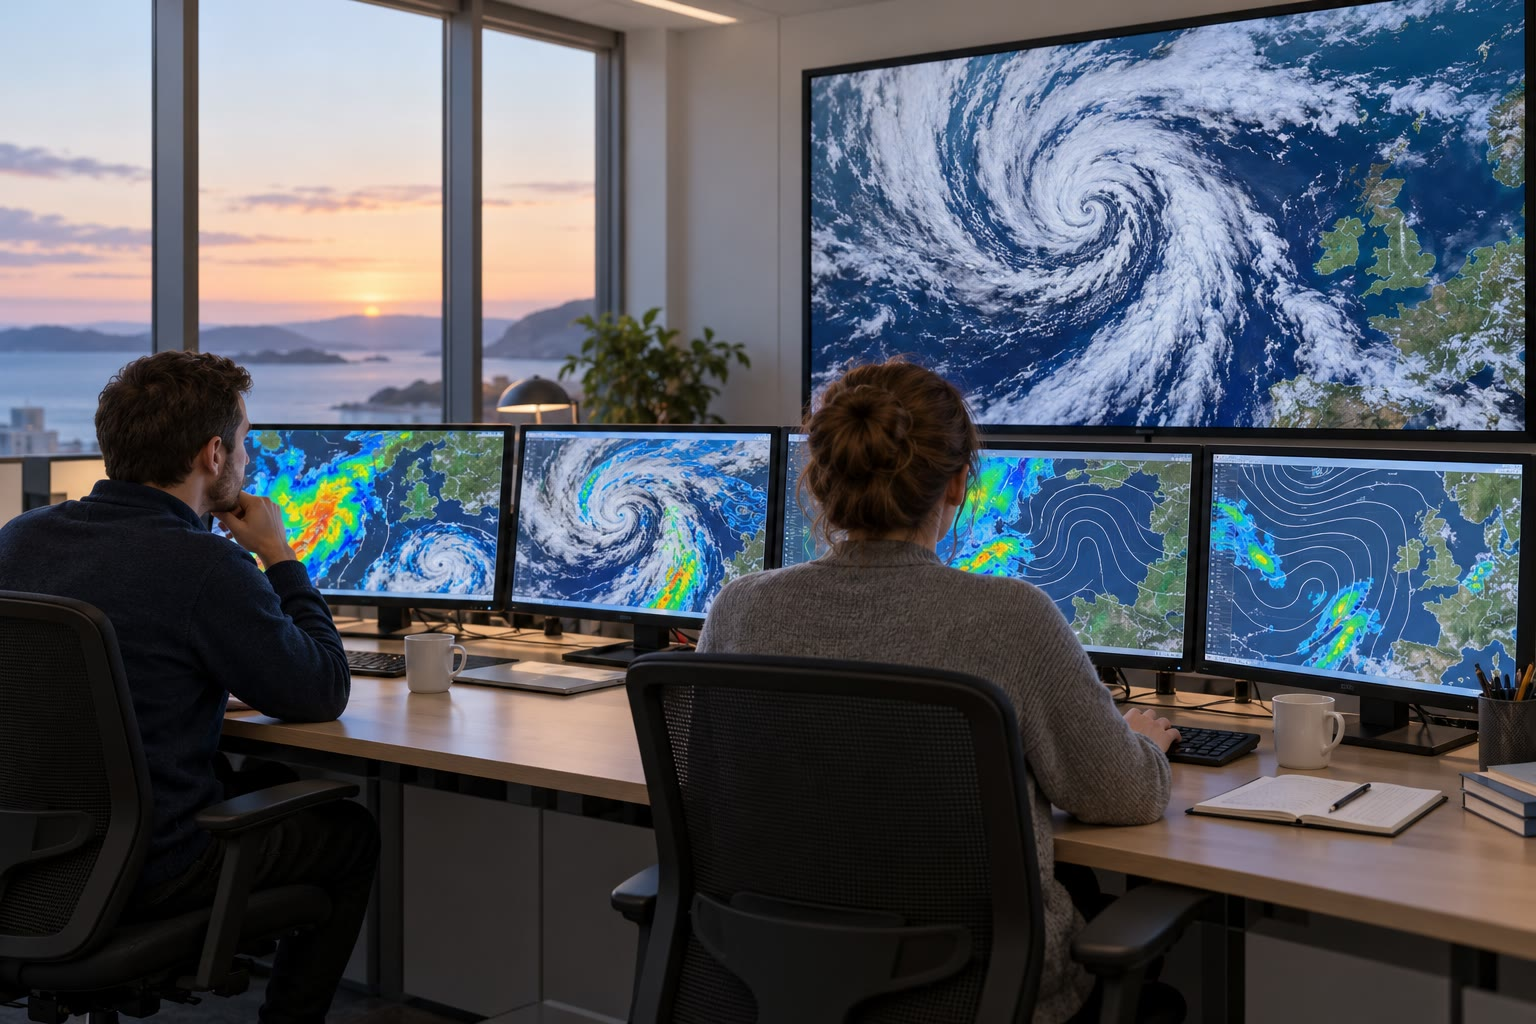
\includegraphics[width=\linewidth]{images/book4/ai/b2-forecast-office.jpg}

{\scriptsize Forecasters at work in front of satellite images and model charts
(AI-generated illustration).}
\end{minipage}
% ledger: ecmwf4:ens, ecmwf4:da, mo:how-forecasts
\end{inthelab}

\section*{Exercises}\label{sec:b2:weather-systems:exercises}

Data for the exercises, unless stated otherwise: $\Omega = \qty{7.292e-5}{s^{-1}}$, $a =
\qty{6371}{km}$, $g = \qty{9.81}{m.s^{-2}}$, $c_p = \qty{1004.5}{J.kg^{-1}.K^{-1}}$, $L =
\qty{2.501e6}{J/kg}$, and the saturation \omterm{def:b2:atmospheric-thermodynamics:moist-air}{vapour pressure} of the exercises of
\cref{ch:b2:atmospheric-thermodynamics}.
% ledger: earth:Trot, earth:Rmean

\begin{exercise}[$\star$]\label{exo:b2:weather-systems:1}
At \ang{50} N a cold front separates air at \qty{275}{K} from air at \qty{281}{K}, and the wind
along it changes by \qty{15}{m/s}. (a) Compute $f$. (b) Compute the slope of the \omterm{def:b2:weather-systems:fronts}{frontal surface},
as 1 in $N$. (c) How far behind the front on the ground does the \omterm{def:b2:weather-systems:fronts}{frontal surface} reach
\qty{1}{km}? (d) What happens to the slope if the temperature contrast doubles at the same wind
shift?
\end{exercise}

\begin{exercise}[$\star$]\label{exo:b2:weather-systems:2}
A warm \omterm{def:b2:weather-systems:fronts}{frontal surface} rises at 1 in 150 and moves at \qty{25}{km/h}. (a) How far ahead of the
front on the ground is the \omterm{def:b2:weather-systems:fronts}{frontal surface} \qty{6}{km} up? (b) An observer sees high cloud form
on it there. How long after does the front reach the observer? (c) Describe the sequence of
clouds the observer sees meanwhile.
\end{exercise}
% ledger: ucar:warm-front

\begin{exercise}[$\star$]\label{exo:b2:weather-systems:3}
On a Northern Hemisphere map, (a) a line with blue triangles on its south-east side runs south-west
from a low; (b) a line with red semicircles on its north side runs east from the same low; (c) a
purple line with both symbols runs from another low to a point where two other fronts start;
(d) a line alternates blue triangles on its south side and red semicircles on its north side.
Name each front, say where the cold air is and which way each moves.
\end{exercise}
% ledger: ucar4:stationary-occluded, nws4:occluded

\begin{exercise}[$\star$]\label{exo:b2:weather-systems:4}
At \ang{45} N in a westerly of \qty{12}{m/s}: (a) compute $\beta$. (b) Compute the phase speed
of waves of \qty{4000}{km} and \qty{8000}{km}. (c) Which way does each move, and how far in a
day?
\end{exercise}

\begin{exercise}[$\star\star$]\label{exo:b2:weather-systems:5}
(a) Show that a \omterm{def:b2:weather-systems:rossby}{Rossby wave} stands still in a westerly $U$ when $\lambda = 2\pi\sqrt{U/\beta}$.
(b) Compute it at \ang{45} N for $U = \qty{12}{m/s}$. (c) How many such waves fit round the
latitude circle? (d) Why would a stronger westerly favour fewer, longer standing waves?
\end{exercise}

\begin{exercise}[$\star\star$]\label{exo:b2:weather-systems:6}
For the Lorenz system: (a) check that $C_+$ is a fixed point by computing the three derivatives
there. (b) By what factor does a small volume of phase space shrink in one time unit? (c) Why
does this not prevent two nearby trajectories from separating?
\end{exercise}

\begin{exercise}[$\star\star$]\label{exo:b2:weather-systems:7}
Take $\lambda = 0.906$ for the Lorenz system and an attractor of size 10. (a) Compute the
doubling time of small errors. (b) How long does an error of \num{e-8} take to reach the size of
the attractor? (c) By how much does a thousandfold smaller initial error delay that moment? What
fraction of the time found in (b) is that?
\end{exercise}
% ledger: nolitia22:lorenz

\begin{exercise}[$\star\star$]\label{exo:b2:weather-systems:8}
A sea at \qty{303}{K} has an outflow at \qty{195}{K}; the disequilibrium is $h_o^* - h^* =
\qty{15}{kJ/kg}$ and $C_k/C_D = 0.9$. (a) Compute the \omterm{prop:b2:weather-systems:pi}{potential intensity}. (b) Compare it with
the threshold of category 5 and with the fastest recent storms. (c) Why do most storms not reach
it?
\end{exercise}
% ledger: gilford21:pi, wk24:scale

\begin{exercise}[$\star\star$]\label{exo:b2:weather-systems:9}
For the storm of \cref{exo:b2:weather-systems:8}: (a) compute the Carnot efficiency of an engine
working between the sea surface and the outflow. (b) Compute the factor $(T_s - T_o)/T_o$ of
\cref{prop:b2:weather-systems:pi} and the ratio of the two. (c) Explain the difference.
\end{exercise}
% ledger: gilford21:pi

\begin{exercise}[$\star\star\star$]\label{exo:b2:weather-systems:10}
(a) Rederive \cref{prop:b2:weather-systems:slope}, keeping the densities exact, and show that
the cold air must lie beneath. (b) Across a frontal zone \qty{50}{km} wide at \ang{45} N the wind
along the front changes by \qty{10}{m/s}. Compute the relative vorticity of the zone and compare
it with $f$. (c) Is the zone cyclonic or anticyclonic?
\end{exercise}

\begin{exercise}[$\star\star\star$]\label{exo:b2:weather-systems:11}
Suppose forecast errors double every 2.4 days, start at \qty{0.5}{K} and are useless at
\qty{6}{K}. (a) Find the horizon of useful forecasts. (b) By what factor must the initial error
shrink each decade to gain a day per decade, if the model were perfect? (c) Experiments find that
a tenfold smaller initial error gains only 4 to 5 days. What doubling time does that imply for
small errors, and what does it say about how small errors grow?
\end{exercise}
% ledger: krish19:predictability, selz22:limit, bauer:day-per-decade

\begin{exercise}[$\star\star\star$]\label{exo:b2:weather-systems:12}
Take \cref{ex:b2:weather-systems:pi} and warm both the sea and the air by \qty{1}{K}, the
relative humidity and the outflow temperature unchanged. (a) Recompute $q_s^*$, $q_a$ and the
disequilibrium. (b) Recompute the \omterm{prop:b2:weather-systems:pi}{potential intensity}. (c) By how many per cent per kelvin does
it rise, and which factor contributes most?
\end{exercise}
% ledger: gilford21:pi

\begin{problem}[{Weekend problem --- How far ahead?}]\label{pb:b2:weather-systems:1}
An invented weather chart at \ang{50} N shows a cold front advancing on a town, with a \omterm{def:b2:weather-systems:rossby}{Rossby
wave} in the jet stream above. The problem follows the front, then the wave, then asks how far
ahead any of it can be forecast. Use the data of the exercises.

\medskip\noindent\textbf{Part I --- The front.}
At 06 UTC the cold front is \qty{480}{km} west of the town, at 12 UTC \qty{390}{km}. Behind it
the air is at \qty{277}{K}, in the warm sector at \qty{285}{K}, and the wind along the front
changes by \qty{16}{m/s} across it.
\begin{enumerate}
  \item Find the speed of the front.
  \item At what time does it reach the town?
  \item Compute $f$ at \ang{50} N.
  \item Compute the slope of the \omterm{def:b2:weather-systems:fronts}{frontal surface}.
  \item How high is the \omterm{def:b2:weather-systems:fronts}{frontal surface} above the town six hours after the front has passed?
  \item How long after the passage does the cold air reach \qty{1.5}{km} above the town?
  \item What weather does the town see as the front passes, and how does the pressure change?
\end{enumerate}

\medskip\noindent\textbf{Part II --- The wave aloft.}
In the jet above, the westerly is \qty{20}{m/s} and the wave has a wavelength of \qty{5000}{km}.
\begin{enumerate}[resume]
  \item Compute $\beta$ at \ang{50} N.
  \item Compute $k$ and $\beta/k^2$.
  \item Find the phase speed of the wave.
  \item How far does a trough move in 24 hours?
  \item Find the wavelength that would stand still in this wind, and how many such waves fit
        round \ang{50} N.
  \item Where, relative to the upper trough, should the surface cyclone deepen?
\end{enumerate}

\medskip\noindent\textbf{Part III --- A toy atmosphere.}
In the figure of the growth of errors in the Lorenz system, the fitted line passes through
about \num{5e-7} at $t = 4$ and \num{3.9e-3} at $t = 14$.
\begin{enumerate}[resume]
  \item From these two readings, compute the growth rate $\lambda$.
  \item Compute the doubling time.
  \item Compare with the published exponent 0.906.
  \item Why does the distance stop growing, at about 15?
  \item How much later does an error ten times smaller reach that size?
\end{enumerate}

\medskip\noindent\textbf{Part IV --- How far ahead?}
Take the doubling time of 2.4 days found for small errors of the forecasts of the 1980s, an
initial error of \qty{0.1}{\celsius} in the temperature at some level, and a forecast that is
useless once the error reaches \qty{3}{\celsius}.
\begin{enumerate}[resume]
  \item How many doublings separate the initial error from the useless one?
  \item How many days does that take?
  \item How many days would halving the initial error gain?
  \item With the earlier estimate of a doubling time of 5 days, what horizon would one find?
  \item Modern experiments find that a tenfold smaller initial error, and even a perfect
        initial state, gains only 4 to 5 days. Why does that suggest that the estimate of
        question 20 is optimistic?
  \item To sum up: how far ahead, in days, could this forecast be useful?
\end{enumerate}
\end{problem}
% ledger: krish19:predictability, selz22:limit, nolitia22:lorenz, ucar:cold-front
